

\subsection{Contact tracing processes}
Figure \ref{fig:tracing} presents the time-varying processes and parameters relating to contact tracing implementation in the model.

\begin{figure}[ht]
    \resizebox{1\textwidth}{!}{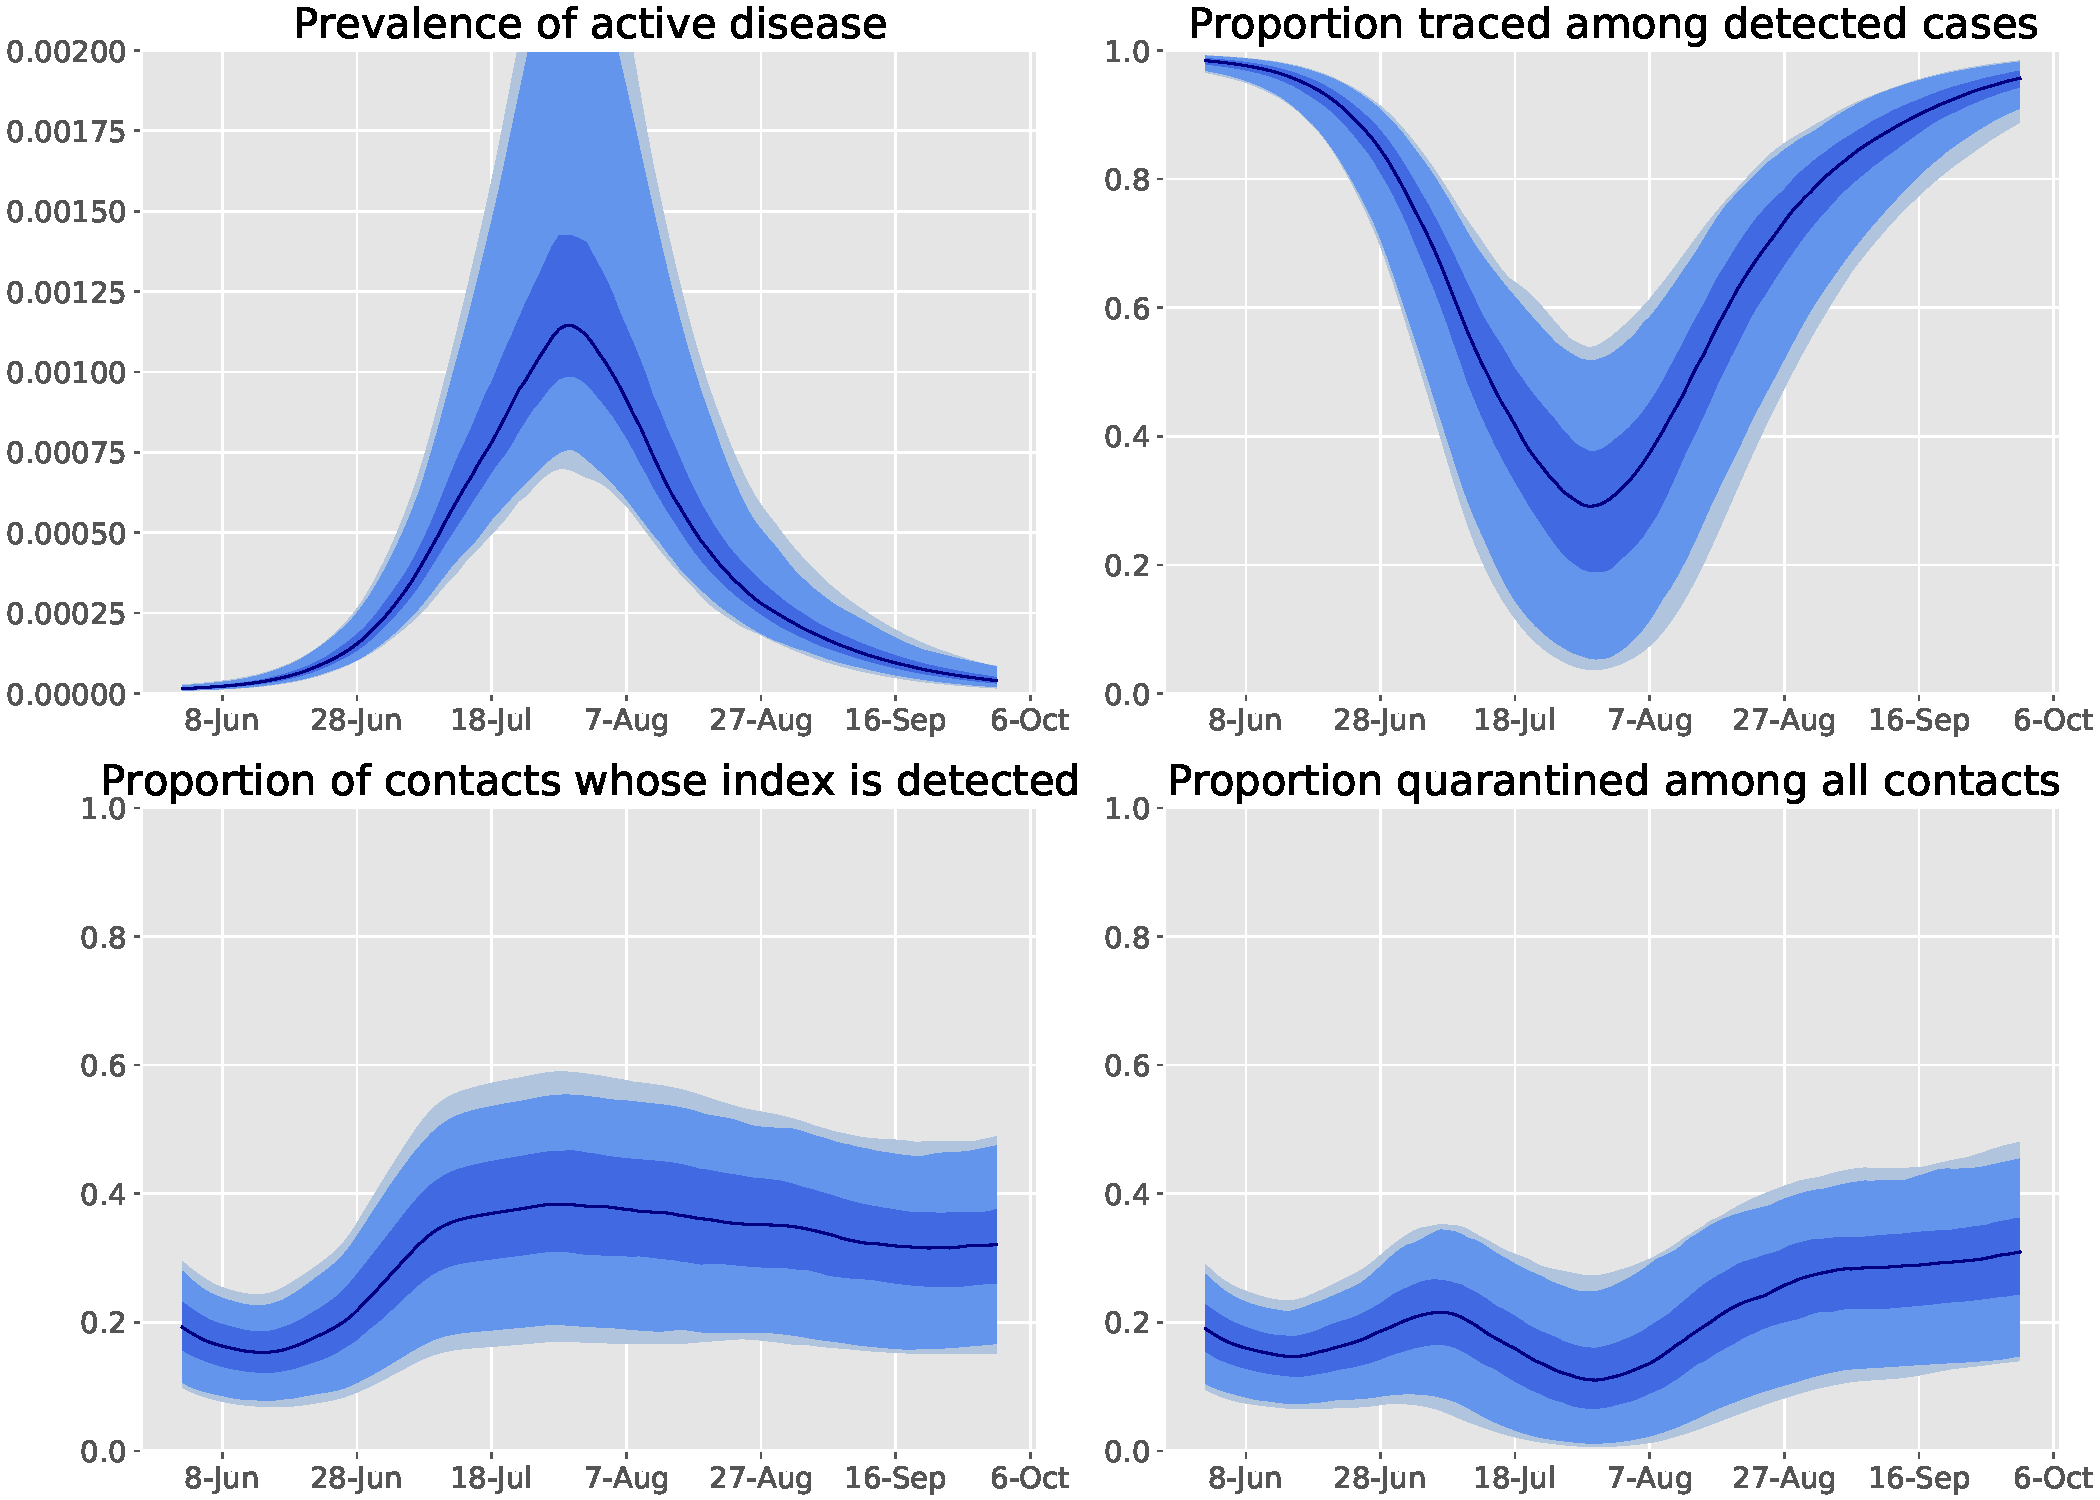
\includegraphics[scale=1]{../covid_19/projects/victoria/results_figures/contact_tracing.png}}
    \caption{\textbf{Contact tracing time-varying processes and parameters.} Upper left panel, modelled prevalence of active COVID-19 episodes (including asymptomatic cases); upper right panel, proportion of contacts traced among contacts of detected cases (declines with increasing prevalence); middle left panel, proportion of symptomatic cases detected (\(CDR(t)\)); middle right panel, proportion of all contacts whose index is detected (scales with proportion of symptomatic cases detected, but includes asymptomatic cases); lower left panel, final proportion of all infected persons quarantined through contact tracing.}
    \label{fig:tracing}
\end{figure}
